\documentclass[twoside]{book}

% Packages required by doxygen
\usepackage{fixltx2e}
\usepackage{calc}
\usepackage{doxygen}
\usepackage[export]{adjustbox} % also loads graphicx
\usepackage{graphicx}
\usepackage[utf8]{inputenc}
\usepackage{makeidx}
\usepackage{multicol}
\usepackage{multirow}
\PassOptionsToPackage{warn}{textcomp}
\usepackage{textcomp}
\usepackage[nointegrals]{wasysym}
\usepackage[table]{xcolor}

% Font selection
\usepackage[T1]{fontenc}
\usepackage[scaled=.90]{helvet}
\usepackage{courier}
\usepackage{amssymb}
\usepackage{sectsty}
\renewcommand{\familydefault}{\sfdefault}
\allsectionsfont{%
  \fontseries{bc}\selectfont%
  \color{darkgray}%
}
\renewcommand{\DoxyLabelFont}{%
  \fontseries{bc}\selectfont%
  \color{darkgray}%
}
\newcommand{\+}{\discretionary{\mbox{\scriptsize$\hookleftarrow$}}{}{}}

% Page & text layout
\usepackage{geometry}
\geometry{%
  a4paper,%
  top=2.5cm,%
  bottom=2.5cm,%
  left=2.5cm,%
  right=2.5cm%
}
\tolerance=750
\hfuzz=15pt
\hbadness=750
\setlength{\emergencystretch}{15pt}
\setlength{\parindent}{0cm}
\setlength{\parskip}{0.2cm}
\makeatletter
\renewcommand{\paragraph}{%
  \@startsection{paragraph}{4}{0ex}{-1.0ex}{1.0ex}{%
    \normalfont\normalsize\bfseries\SS@parafont%
  }%
}
\renewcommand{\subparagraph}{%
  \@startsection{subparagraph}{5}{0ex}{-1.0ex}{1.0ex}{%
    \normalfont\normalsize\bfseries\SS@subparafont%
  }%
}
\makeatother

% Headers & footers
\usepackage{fancyhdr}
\pagestyle{fancyplain}
\fancyhead[LE]{\fancyplain{}{\bfseries\thepage}}
\fancyhead[CE]{\fancyplain{}{}}
\fancyhead[RE]{\fancyplain{}{\bfseries\leftmark}}
\fancyhead[LO]{\fancyplain{}{\bfseries\rightmark}}
\fancyhead[CO]{\fancyplain{}{}}
\fancyhead[RO]{\fancyplain{}{\bfseries\thepage}}
\fancyfoot[LE]{\fancyplain{}{}}
\fancyfoot[CE]{\fancyplain{}{}}
\fancyfoot[RE]{\fancyplain{}{\bfseries\scriptsize Generated on Sat Sep 26 2015 12\+:28\+:03 for Deduplicator by Doxygen }}
\fancyfoot[LO]{\fancyplain{}{\bfseries\scriptsize Generated on Sat Sep 26 2015 12\+:28\+:03 for Deduplicator by Doxygen }}
\fancyfoot[CO]{\fancyplain{}{}}
\fancyfoot[RO]{\fancyplain{}{}}
\renewcommand{\footrulewidth}{0.4pt}
\renewcommand{\chaptermark}[1]{%
  \markboth{#1}{}%
}
\renewcommand{\sectionmark}[1]{%
  \markright{\thesection\ #1}%
}

% Indices & bibliography
\usepackage{natbib}
\usepackage[titles]{tocloft}
\setcounter{tocdepth}{3}
\setcounter{secnumdepth}{5}
\makeindex

% Hyperlinks (required, but should be loaded last)
\usepackage{ifpdf}
\ifpdf
  \usepackage[pdftex,pagebackref=true]{hyperref}
\else
  \usepackage[ps2pdf,pagebackref=true]{hyperref}
\fi
\hypersetup{%
  colorlinks=true,%
  linkcolor=blue,%
  citecolor=blue,%
  unicode%
}

% Custom commands
\newcommand{\clearemptydoublepage}{%
  \newpage{\pagestyle{empty}\cleardoublepage}%
}


%===== C O N T E N T S =====

\begin{document}

% Titlepage & ToC
\hypersetup{pageanchor=false,
             bookmarks=true,
             bookmarksnumbered=true,
             pdfencoding=unicode
            }
\pagenumbering{roman}
\begin{titlepage}
\vspace*{7cm}
\begin{center}%
{\Large Deduplicator \\[1ex]\large 0.\+1 }\\
\vspace*{1cm}
{\large Generated by Doxygen 1.8.9.1}\\
\vspace*{0.5cm}
{\small Sat Sep 26 2015 12:28:03}\\
\end{center}
\end{titlepage}
\clearemptydoublepage
\tableofcontents
\clearemptydoublepage
\pagenumbering{arabic}
\hypersetup{pageanchor=true}

%--- Begin generated contents ---
\chapter{Deduplicator}
\label{md__r_e_a_d_m_e}
\hypertarget{md__r_e_a_d_m_e}{}
Simple tool to safely and efficiently remove duplicate files from a local filesystem

Requires boost\+::filesystem to build

Requires B\+M\+C\+A header-\/only library to build (\href{https://github.com/Ranind/BMCA}{\tt https\+://github.\+com/\+Ranind/\+B\+M\+C\+A})

Compile with\+: g++ $\ast$.cpp -\/std=c++11 -\/lboost\+\_\+system -\/lboost\+\_\+filesystem 
\chapter{Class Index}
\section{Class List}
Here are the classes, structs, unions and interfaces with brief descriptions\+:\begin{DoxyCompactList}
\item\contentsline{section}{\hyperlink{struct_file}{File} }{\pageref{struct_file}}{}
\item\contentsline{section}{\hyperlink{struct_file_bucket}{File\+Bucket} }{\pageref{struct_file_bucket}}{}
\end{DoxyCompactList}

\chapter{File Index}
\section{File List}
Here is a list of all files with brief descriptions\+:\begin{DoxyCompactList}
\item\contentsline{section}{\hyperlink{main_8cpp}{main.\+cpp} }{\pageref{main_8cpp}}{}
\end{DoxyCompactList}

\chapter{Class Documentation}
\hypertarget{struct_file}{}\section{File Struct Reference}
\label{struct_file}\index{File@{File}}
\subsection*{Public Member Functions}
\begin{DoxyCompactItemize}
\item 
\hyperlink{struct_file_aafc278d5a9d7437481bb462c3e8d78b4}{File} (boost\+::filesystem\+::path p, int s)
\item 
bool \hyperlink{struct_file_acce9541acd27b8d5ab744127e014587c}{operator==} (const \hyperlink{struct_file}{File} \&rhs)
\end{DoxyCompactItemize}
\subsection*{Public Attributes}
\begin{DoxyCompactItemize}
\item 
boost\+::filesystem\+::path \hyperlink{struct_file_ab546c52089e48bee96c9a3e4a0433bf4}{path}
\item 
int \hyperlink{struct_file_abec73ae2a96ee8136ba14a49fec88b25}{size}
\end{DoxyCompactItemize}


\subsection{Detailed Description}


Definition at line 10 of file main.\+cpp.



\subsection{Constructor \& Destructor Documentation}
\hypertarget{struct_file_aafc278d5a9d7437481bb462c3e8d78b4}{}\index{File@{File}!File@{File}}
\index{File@{File}!File@{File}}
\subsubsection[{File}]{\setlength{\rightskip}{0pt plus 5cm}File\+::\+File (
\begin{DoxyParamCaption}
\item[{boost\+::filesystem\+::path}]{p, }
\item[{int}]{s}
\end{DoxyParamCaption}
)\hspace{0.3cm}{\ttfamily [inline]}}\label{struct_file_aafc278d5a9d7437481bb462c3e8d78b4}


Definition at line 14 of file main.\+cpp.



\subsection{Member Function Documentation}
\hypertarget{struct_file_acce9541acd27b8d5ab744127e014587c}{}\index{File@{File}!operator==@{operator==}}
\index{operator==@{operator==}!File@{File}}
\subsubsection[{operator==}]{\setlength{\rightskip}{0pt plus 5cm}bool File\+::operator== (
\begin{DoxyParamCaption}
\item[{const {\bf File} \&}]{rhs}
\end{DoxyParamCaption}
)\hspace{0.3cm}{\ttfamily [inline]}}\label{struct_file_acce9541acd27b8d5ab744127e014587c}


Definition at line 19 of file main.\+cpp.



\subsection{Member Data Documentation}
\hypertarget{struct_file_ab546c52089e48bee96c9a3e4a0433bf4}{}\index{File@{File}!path@{path}}
\index{path@{path}!File@{File}}
\subsubsection[{path}]{\setlength{\rightskip}{0pt plus 5cm}boost\+::filesystem\+::path File\+::path}\label{struct_file_ab546c52089e48bee96c9a3e4a0433bf4}


Definition at line 11 of file main.\+cpp.

\hypertarget{struct_file_abec73ae2a96ee8136ba14a49fec88b25}{}\index{File@{File}!size@{size}}
\index{size@{size}!File@{File}}
\subsubsection[{size}]{\setlength{\rightskip}{0pt plus 5cm}int File\+::size}\label{struct_file_abec73ae2a96ee8136ba14a49fec88b25}


Definition at line 12 of file main.\+cpp.



The documentation for this struct was generated from the following file\+:\begin{DoxyCompactItemize}
\item 
\hyperlink{main_8cpp}{main.\+cpp}\end{DoxyCompactItemize}

\hypertarget{struct_file_bucket}{}\section{File\+Bucket Struct Reference}
\label{struct_file_bucket}\index{File\+Bucket@{File\+Bucket}}
\subsection*{Public Member Functions}
\begin{DoxyCompactItemize}
\item 
\hyperlink{struct_file_bucket_afc1e5378909a2241237c113c5d83e410}{File\+Bucket} ()
\item 
\hyperlink{struct_file_bucket_aa6b5213e228054000ef4373407e39e58}{File\+Bucket} (int \hyperlink{struct_file_bucket_a16f787c14b9b69c959374749f70bb80a}{size})
\item 
void \hyperlink{struct_file_bucket_a44e2797122359f1b1f7cb67a0f02e2ce}{add\+File} (boost\+::filesystem\+::path path)
\item 
bool \hyperlink{struct_file_bucket_a97ba88a917daa112da2fcd008082a0f4}{operator$<$} (const \hyperlink{struct_file_bucket}{File\+Bucket} \&rhs)
\item 
bool \hyperlink{struct_file_bucket_ac5f5769f6643b0f078a49c80f48233ff}{operator==} (const \hyperlink{struct_file_bucket}{File\+Bucket} \&rhs)
\end{DoxyCompactItemize}
\subsection*{Public Attributes}
\begin{DoxyCompactItemize}
\item 
int \hyperlink{struct_file_bucket_a16f787c14b9b69c959374749f70bb80a}{size}
\item 
std\+::vector$<$ \hyperlink{struct_file}{File} $>$ \hyperlink{struct_file_bucket_a4da87f8307c3d3b6b477b6277897d5b9}{files}
\end{DoxyCompactItemize}


\subsection{Detailed Description}


Definition at line 40 of file main.\+cpp.



\subsection{Constructor \& Destructor Documentation}
\hypertarget{struct_file_bucket_afc1e5378909a2241237c113c5d83e410}{}\index{File\+Bucket@{File\+Bucket}!File\+Bucket@{File\+Bucket}}
\index{File\+Bucket@{File\+Bucket}!File\+Bucket@{File\+Bucket}}
\subsubsection[{File\+Bucket}]{\setlength{\rightskip}{0pt plus 5cm}File\+Bucket\+::\+File\+Bucket (
\begin{DoxyParamCaption}
{}
\end{DoxyParamCaption}
)\hspace{0.3cm}{\ttfamily [inline]}}\label{struct_file_bucket_afc1e5378909a2241237c113c5d83e410}


Definition at line 44 of file main.\+cpp.

\hypertarget{struct_file_bucket_aa6b5213e228054000ef4373407e39e58}{}\index{File\+Bucket@{File\+Bucket}!File\+Bucket@{File\+Bucket}}
\index{File\+Bucket@{File\+Bucket}!File\+Bucket@{File\+Bucket}}
\subsubsection[{File\+Bucket}]{\setlength{\rightskip}{0pt plus 5cm}File\+Bucket\+::\+File\+Bucket (
\begin{DoxyParamCaption}
\item[{int}]{size}
\end{DoxyParamCaption}
)\hspace{0.3cm}{\ttfamily [inline]}}\label{struct_file_bucket_aa6b5213e228054000ef4373407e39e58}


Definition at line 48 of file main.\+cpp.



\subsection{Member Function Documentation}
\hypertarget{struct_file_bucket_a44e2797122359f1b1f7cb67a0f02e2ce}{}\index{File\+Bucket@{File\+Bucket}!add\+File@{add\+File}}
\index{add\+File@{add\+File}!File\+Bucket@{File\+Bucket}}
\subsubsection[{add\+File}]{\setlength{\rightskip}{0pt plus 5cm}void File\+Bucket\+::add\+File (
\begin{DoxyParamCaption}
\item[{boost\+::filesystem\+::path}]{path}
\end{DoxyParamCaption}
)\hspace{0.3cm}{\ttfamily [inline]}}\label{struct_file_bucket_a44e2797122359f1b1f7cb67a0f02e2ce}


Definition at line 52 of file main.\+cpp.

\hypertarget{struct_file_bucket_a97ba88a917daa112da2fcd008082a0f4}{}\index{File\+Bucket@{File\+Bucket}!operator$<$@{operator$<$}}
\index{operator$<$@{operator$<$}!File\+Bucket@{File\+Bucket}}
\subsubsection[{operator$<$}]{\setlength{\rightskip}{0pt plus 5cm}bool File\+Bucket\+::operator$<$ (
\begin{DoxyParamCaption}
\item[{const {\bf File\+Bucket} \&}]{rhs}
\end{DoxyParamCaption}
)\hspace{0.3cm}{\ttfamily [inline]}}\label{struct_file_bucket_a97ba88a917daa112da2fcd008082a0f4}


Definition at line 56 of file main.\+cpp.

\hypertarget{struct_file_bucket_ac5f5769f6643b0f078a49c80f48233ff}{}\index{File\+Bucket@{File\+Bucket}!operator==@{operator==}}
\index{operator==@{operator==}!File\+Bucket@{File\+Bucket}}
\subsubsection[{operator==}]{\setlength{\rightskip}{0pt plus 5cm}bool File\+Bucket\+::operator== (
\begin{DoxyParamCaption}
\item[{const {\bf File\+Bucket} \&}]{rhs}
\end{DoxyParamCaption}
)\hspace{0.3cm}{\ttfamily [inline]}}\label{struct_file_bucket_ac5f5769f6643b0f078a49c80f48233ff}


Definition at line 60 of file main.\+cpp.



\subsection{Member Data Documentation}
\hypertarget{struct_file_bucket_a4da87f8307c3d3b6b477b6277897d5b9}{}\index{File\+Bucket@{File\+Bucket}!files@{files}}
\index{files@{files}!File\+Bucket@{File\+Bucket}}
\subsubsection[{files}]{\setlength{\rightskip}{0pt plus 5cm}std\+::vector$<${\bf File}$>$ File\+Bucket\+::files}\label{struct_file_bucket_a4da87f8307c3d3b6b477b6277897d5b9}


Definition at line 42 of file main.\+cpp.

\hypertarget{struct_file_bucket_a16f787c14b9b69c959374749f70bb80a}{}\index{File\+Bucket@{File\+Bucket}!size@{size}}
\index{size@{size}!File\+Bucket@{File\+Bucket}}
\subsubsection[{size}]{\setlength{\rightskip}{0pt plus 5cm}int File\+Bucket\+::size}\label{struct_file_bucket_a16f787c14b9b69c959374749f70bb80a}


Definition at line 41 of file main.\+cpp.



The documentation for this struct was generated from the following file\+:\begin{DoxyCompactItemize}
\item 
\hyperlink{main_8cpp}{main.\+cpp}\end{DoxyCompactItemize}

\chapter{File Documentation}
\hypertarget{main_8cpp}{}\section{main.\+cpp File Reference}
\label{main_8cpp}\index{main.\+cpp@{main.\+cpp}}
{\ttfamily \#include $<$iostream$>$}\\*
{\ttfamily \#include $<$string$>$}\\*
{\ttfamily \#include $<$vector$>$}\\*
{\ttfamily \#include $<$boost/filesystem.\+hpp$>$}\\*
{\ttfamily \#include $<$boost/format.\+hpp$>$}\\*
{\ttfamily \#include \char`\"{}bmca/consoleui.\+h\char`\"{}}\\*
{\ttfamily \#include \char`\"{}A\+V\+L\+Tree.\+h\char`\"{}}\\*
Include dependency graph for main.\+cpp\+:
\nopagebreak
\begin{figure}[H]
\begin{center}
\leavevmode
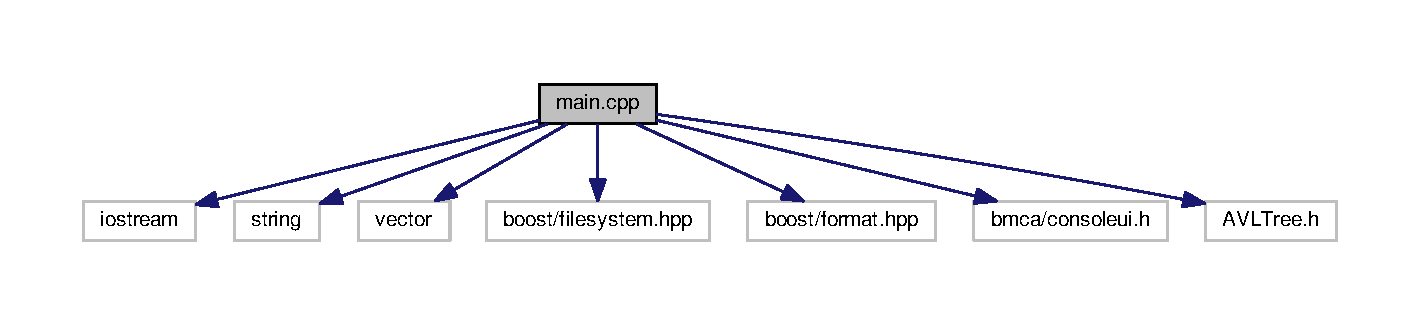
\includegraphics[width=350pt]{main_8cpp__incl}
\end{center}
\end{figure}
\subsection*{Classes}
\begin{DoxyCompactItemize}
\item 
struct \hyperlink{struct_file}{File}
\item 
struct \hyperlink{struct_file_bucket}{File\+Bucket}
\end{DoxyCompactItemize}
\subsection*{Functions}
\begin{DoxyCompactItemize}
\item 
void \hyperlink{main_8cpp_a1c024cff868e015ff5faa282364a6302}{filter\+Duplicates} (std\+::vector$<$ boost\+::filesystem\+::path $>$ \&paths, A\+V\+L\+Node$<$ \hyperlink{struct_file_bucket}{File\+Bucket} $>$ $\ast$file)
\begin{DoxyCompactList}\small\item\em Filters out duplicate paths, if remove\+Duplicates is true it will remove those files, if false it will only keep them (gives a list of files to delete for example) \end{DoxyCompactList}\item 
void \hyperlink{main_8cpp_a1bc69b1b6f62d721f14ed9c03555a9c8}{scan\+Files} (A\+V\+L\+Tree$<$ \hyperlink{struct_file_bucket}{File\+Bucket} $>$ \&files, std\+::string root\+Path, bool recursive)
\begin{DoxyCompactList}\small\item\em Builds file objects for all files contained within the given directory. \end{DoxyCompactList}\item 
int \hyperlink{main_8cpp_a3c04138a5bfe5d72780bb7e82a18e627}{main} (int argc, char $\ast$$\ast$argv)
\end{DoxyCompactItemize}


\subsection{Function Documentation}
\hypertarget{main_8cpp_a1c024cff868e015ff5faa282364a6302}{}\index{main.\+cpp@{main.\+cpp}!filter\+Duplicates@{filter\+Duplicates}}
\index{filter\+Duplicates@{filter\+Duplicates}!main.\+cpp@{main.\+cpp}}
\subsubsection[{filter\+Duplicates}]{\setlength{\rightskip}{0pt plus 5cm}void filter\+Duplicates (
\begin{DoxyParamCaption}
\item[{std\+::vector$<$ boost\+::filesystem\+::path $>$ \&}]{paths, }
\item[{A\+V\+L\+Node$<$ {\bf File\+Bucket} $>$ $\ast$}]{file}
\end{DoxyParamCaption}
)}\label{main_8cpp_a1c024cff868e015ff5faa282364a6302}


Filters out duplicate paths, if remove\+Duplicates is true it will remove those files, if false it will only keep them (gives a list of files to delete for example) 



Definition at line 66 of file main.\+cpp.

\hypertarget{main_8cpp_a3c04138a5bfe5d72780bb7e82a18e627}{}\index{main.\+cpp@{main.\+cpp}!main@{main}}
\index{main@{main}!main.\+cpp@{main.\+cpp}}
\subsubsection[{main}]{\setlength{\rightskip}{0pt plus 5cm}int main (
\begin{DoxyParamCaption}
\item[{int}]{argc, }
\item[{char $\ast$$\ast$}]{argv}
\end{DoxyParamCaption}
)}\label{main_8cpp_a3c04138a5bfe5d72780bb7e82a18e627}


Definition at line 127 of file main.\+cpp.

\hypertarget{main_8cpp_a1bc69b1b6f62d721f14ed9c03555a9c8}{}\index{main.\+cpp@{main.\+cpp}!scan\+Files@{scan\+Files}}
\index{scan\+Files@{scan\+Files}!main.\+cpp@{main.\+cpp}}
\subsubsection[{scan\+Files}]{\setlength{\rightskip}{0pt plus 5cm}void scan\+Files (
\begin{DoxyParamCaption}
\item[{A\+V\+L\+Tree$<$ {\bf File\+Bucket} $>$ \&}]{files, }
\item[{std\+::string}]{root\+Path, }
\item[{bool}]{recursive}
\end{DoxyParamCaption}
)}\label{main_8cpp_a1bc69b1b6f62d721f14ed9c03555a9c8}


Builds file objects for all files contained within the given directory. 



Definition at line 84 of file main.\+cpp.


\hypertarget{_r_e_a_d_m_e_8md}{}\section{R\+E\+A\+D\+M\+E.\+md File Reference}
\label{_r_e_a_d_m_e_8md}\index{R\+E\+A\+D\+M\+E.\+md@{R\+E\+A\+D\+M\+E.\+md}}

%--- End generated contents ---

% Index
\backmatter
\newpage
\phantomsection
\clearemptydoublepage
\addcontentsline{toc}{chapter}{Index}
\printindex

\end{document}
